\chapter{State-of-the-Art}\label{chap:state-art}
In the demand for an effective, high-quality approach to the analysis of isolates from infected animals, molecular studies help to investigate characteristics of the sample. Genome analysis has become an integral part of animal disease surveillance, especially since the advent of high-throughput sequencing technologies in the last 15 years. Next-generation techniques and applications are described below, the state of the art in poxvirus and avian influenza virus detection and analysis, and lastly the drawbacks of the methods discussed.

\section{High-throughput Technologies in Genomics and Virology}
When comparing DNA sequencing technologies, there are differences in speed, throughput and volume of sequences. The term ''next-generation'' in NGS used to describe newer technologies in the field implies a next step in the evolution of sequencing technologies. As sequencing machine technologies evolve rapidly, there are gradations such as ''second-generation'' and ''third-generation''. Following the original 1977 Sanger sequencing method using radioactivity and gels, second-generation sequencers are advancements of Sanger sequencing that uses sequencing by synthesis~\cite{mardis2008next}. In second-generation methods, reactions run in parallel and drastically reduce overall costs compared to Sanger sequencing. They produce short sequence reads length and are able to detect reads without using electrophoresis. Reads are equal to single fragments of DNA or RNA.
Third-generation sequencing technologies typically generate longer primary reads of DNA (and RNA) molecules while maintaining the massive parallelism of the technology and taking advantage of this benefit~\cite{slatko2018overview}. The nowadays most commonly used next-generation technologies for DNA sequencing and their applications are described below.

\subsection{NGS Platforms and Applications}
By far the biggest player in the field of DNA sequencing is the Illumina platform, first developed by Solexa and Lync Therapeutics~\cite{illumina2015introduction}. Illumina sequencing is based on bridge amplification, which creates clusters of copies of each DNA fragment. This technique involves repeated synthesis reactions with proprietary modified nucleotides containing a different fluorescent label for each of the four bases A, T, C and G. The reactions are performed over 300 or more rounds, and fluorescent detection allows for faster detection through direct imaging. An Illumina sequencer outputs data in the form of sequence reads, which are short DNA fragments ranging from 50 to 600 base pairs in length depending on the specific instrument and protocol used~\cite{illumina2015introduction, slatko2018overview, mardis2008next}. The output data from an Illumina sequencer typically is in the form of raw sequence files in FASTQ format, which contain the base calls and corresponding quality scores for each read. These reads can be used for downstream analyses such as viral genome assembly and variant calling.

Oxford Nanopore Technologies (ONT) is a third-generation paradigm shifting sequencing technology. It measures changes in ionic current across membranes as single-stranded DNA nucleotides pass through a nanopore~\cite{jain2016oxford}. Nanopore-based DNA sequencing technologies are purchasable as a portable, small MinION (ONT) device, allowing experts to use it for applications where space requirements or portability are important~\cite{greninger2015rapid, jain2016oxford}. The cyclic mode of sequencing used in second-generation approaches is replaced by sequencing in real-time with read lengths of up to 10,000 basepairs~\cite{jain2016oxford}. Despite its advantages, the main caveat of ONT is its relatively high error rate compared to other HTS methods~\cite{fu2019comparative}. This makes ONT less suitable for single-nucleotide variant analysis that is required in some diagnostic applications~\cite{bowden2019sequencing, stefan2022comparison}.

Other frequently used second-generation platforms are Roche/454 sequencing, Ion Torrent (Thermo Fisher) technology and SOLiD (Sequencing by Oligonucleotide Ligation and Detection). Third-generation platforms include single molecule real-time sequencing (SMRT) by PacBio and nanopore sequencing~\cite{rhoads2015pacbio}. 

\begin{figure}
	\centering
	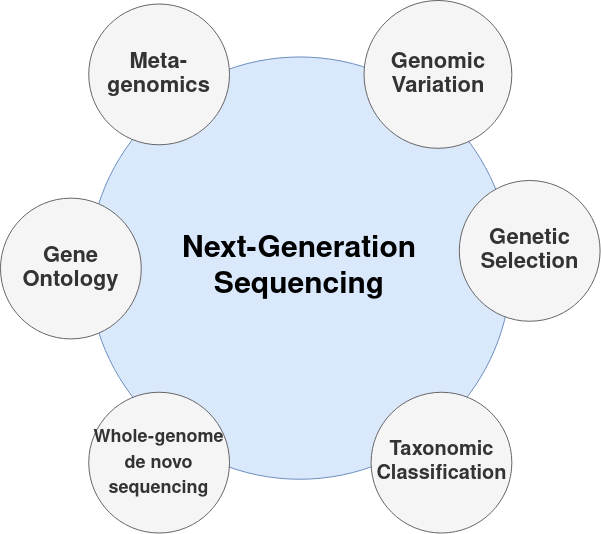
\includegraphics[width=0.5\textwidth]{media/2-ngs.png}
	\caption{Overview of next-generation sequencing technology applications in virology.}
	\label{fig:2-ngs}
\end{figure} 

As NGS platforms are widely used in biomedical and clinical contexts, some of the most important applications in diagnostic virology are depicted in Figure~\ref{fig:2-ngs}. In virology, metagenomics can be used to identify viruses in complex clinical samples~\cite{chiu2019clinical}. It allows for the detection of known and novel viruses without prior knowledge of the infectious agent. Metagenomics involves the sequencing of all genetic material in a sample, including viral genomes, to identify the presence of viruses. Once a virus is identified, genomic variation refers to differences in the DNA sequence of a virus between different strains or isolates. These variants can be used for tracking the spread of an outbreak, identification of sources of an infection, or determination of the level of virus virulence~\cite{capobianchi2013next}. Variant detection is only possible with NGS data, as they provide insight to the genome on a nearly every-base level and allow to reliably interpret and identify the many different possible variants~\cite{koboldt2013next}. \\ 
Genetic selection describes to the process by which certain viral strains become more prevalent in a population over time due to selective pressures. In diagnostic virology, genetic selection is used to track the evolution of a virus in the course of time and determine which strains are most likely to cause outbreaks or epidemics. This is of special interest in the backtracing of infected animals to know where the virus came from. Using gene ontology, functions and interactions of genes are described. This is crucial to identify the genes responsible for specific viral functions and to understand how these functions contribute to viral pathogenesis. \\
Based on their genetic and structural characteristics, viruses are classified to existing systems, called taxonomic classification. This clustering analysis can be used for the type identification of a virus causing infections and determination of its potential for transmission and pathogenicity~\cite{dutilh2021perspective}.\\
Whole-genome de novo sequencing is the sequencing of an entire viral genome without prior knowledge of its genetic sequence. Similar to metagenomics, this technique can be used to identify novel viruses, to study mutations in viral genomes and to track the evolution of a virus over time~\cite{slatko2018overview}.

\subsection{Detection of Viral Pathogens}
For NGS methods to be a viable tool in diagnosis and analysis of viral animal diseases, the methods must be efficient and reliable. Almost all downstream analyses depend on the data obtained by sequencing, so it is imperative to choose the most appropriate method for each application. Metagenomic-based approaches use whole-genome sequencing to characterise viral diversity in animal, human and environmental samples. The detection of rare and novel infectious pathogens and the study of mutations in the genome are crucial for developing a deeper understanding of livestock viromes and potential zoonotic agents. In addition, NGS has been shown to detect non-culturable organisms as well as co-infections that have not been detected using traditional microbiological approaches~\cite{cantalupo2019detecting}. Metagenome sequencing often relies on a low number of pathogenic reads to detect and to make diagnostic calls. As sequencing depth directly influences genome coverage that can be obtained, the optimal amount of data to cover the complete genome is necessary. It has been shown that for a full virus genome to be represented, NGS data generated from ribo-depleted total RNA with a minimum length of one million high-quality reads works best~\cite{visser2016next}. Nevertheless, validation pipelines and confirmatory tests are needed for NGS approaches to pathogen detection~\cite{minogue2019next}.

\subsection{Data Analysis Issues}
Since the surveillance of viral animal diseases with NGS is advancing rapidly, it is important that regions and health organizations that experience high damage of viral outbreaks but do not have their own facilities and know-how have access to the needed tools and knowledge. Costs for NGS sequencers are still high and the access to appropriate laboratories is not given everywhere. Networks like VETLAB and standardisation of techniques, for example freely available and published by the WOAH, can enable professionals worldwide independent of their equipment on site. In the scope of the ZODIAC project, this aspect is addressed by providing protocols for each step from taking samples of potentially infected animals to the detailed analysis and derived actions~\cite{zodiac2021}.

NGS methods themselves have downsides that need to be considered when applying these techniques. Generally, chimerical sequences are formed during sequencing, which may be interpreted as false positives for novel organisms. Chimeric products are artifacts originating from joining sequences and are represented by point mutations, insertions and deletions. Chimera formation also occurs during PCR amplification~\cite{zylstra1998pcr}.\\
During bioinformatics analysis steps using algorithms with computationally expensive steps, the choice of the algorithm as well as its configuration settings have huge impact on the final results obtained. This includes algorithms in steps such as filtering for quality, clustering and sequence classification~\cite{kopylova2016open}. The cleaning step or filtering phase eliminates low-quality reads from the dataset, whereas the error correction process distinguishes true variants from those caused by experimental noise. This is based on the concept that errors occur randomly with low frequency, while true mutations tend to be clustered, and their frequency can be measured~\cite{zagordi2010error}. Longer reads avoid this problem because contigs must not be assembled in the first place, avoiding clustering and filtering errors. This is why the shift in third-generation and later sequencing platforms is towards longer reads again. Due to the relatively high error rates of HTS technologies, that base on the sequencing process itself, polymerase chain reaction (PCR) amplification of the viral material, and reverse transcription of viral RNA to cDNA, it is crucial to include quality checks and filtering steps when using the HTS data~\cite{beerenwinkel2012challenges}. \\
Each application of software with NGS data requires expertise in resolving limitations and drawbacks of specific methods. This in turn requires skills and experience in the field and the careful interpretation of results. Still, NGS provides a large pool of methods which eases this task, although available algorithms for genome assembly and amplicon analysis have drawbacks and limitations~\cite{finotello2012comparative}.

\section{Poxvirus Analysis}
In the following, current approaches to analyse NGS data of poxviruses are described. To get into the topic, the characteristics of poxviruses are examined.

\subsection{Poxviruses}
Throughout human history, poxviruses have played a significant role with variola being the most notorious as it is the causative agent of smallpox. Smallpox has been described in Chinese texts dating back to the 4th Century AD, and evidence of pox-like scars found on Egyptian mummies suggests the disease may have existed as far back as the 2nd millennium BC~\cite{fenner1988history}. The discovery of a vaccine for smallpox made it the first disease to be eradicated by human efforts, and variola was the first human virus to be successfully eliminated~\cite{fenner2000adventures}. Modern vaccinology owes its origins to Edward Jenner's discovery in the late 18th century that zoonotic infections with the ''cowpox virus'' provided immunity to smallpox~\cite{fenner1988history}. Furthermore, vaccinia virus, which is now used for smallpox vaccination, was the first animal virus to be observed using electron microscopy and the first to be utilized as a vector for transporting foreign genes into animals. This is why poxviruses are among the best-known viruses. \\
The family of poxviruses, \textit{Poxviridae}, is a family of double-stranded DNA viruses. Its natural hosts are vertebrates and arthropods and there are currently 83 species within 22 genera in this family. The family is divided into two subfamilies, \textit{Entemopoxvirinae} (insect-infecting viruses) and \textit{Chordopoxvirinae} (vertebrate-infecting viruses). \\
Historically, poxviruses were classified based on disease symptoms and the animal species that was infected. Humans, cows, sheep, goats, horses and pigs have been studied to determine not only clinical symptoms but with the aim to classify poxviruses. This genus classisification has been confirmed by recent comparative genome analysis~\cite{gubser2004poxvirus}. Symptoms of disease caused by a poxvirus infection are skin lesions that can differ in size. Depending on the type of poxvirus, the papules can vary from small and pearly papules in infections of lumpy skin disease virus (LSDV) to larger crusts and spread generalized pustules in infections with the variola virus. Other general symptoms include fever, headache and rash.

\renewcommand{\arraystretch}{1.4}
\begin{table}[ht!]
	\begin{tabular}{lll}
	\hline
	\textbf{Genus}      & \textbf{Virus Species}                          & \textbf{Natural Hosts}                      \\ \hline
	Avipoxvirus         & Canarypox virus                                 & Songbirds 									\\ 
						& Fowlpox virus                                   & Chickens, turkeys                           \\ \hline
	Capripoxvirus       & Sheep pox virus                                 & Sheep                                       \\
	                    & Lumpy skin disease virus                        & Cattle                                      \\ \hline
	Centapoxvirus       & Yokapox virus\textsuperscript{1}                & Humans, mosquitoes                          \\ \hline
	Cervidpoxvirus      & Deerpox virus                                   & Deer                                        \\ \hline
	Crocodylidpoxvirus  & Crocodilepox virus                              & Crocodiles                                  \\ \hline
	Leporipoxvirus      & Myxoma virus                                    & Rabbits, hares                              \\ \hline
	Molluscipoxvirus    & Molluscum contagiosum virus\textsuperscript{1}  & Humans, primates, birds, dogs               \\ \hline
	Orthopoxvirus       & Variola virus (Smallpox)                        & Humans (eradicated)                         \\ 
						& Mpox virus\textsuperscript{1}                   & Humans, primates                            \\ 
						& Cowpox virus\textsuperscript{1}                 & Humans, cats, cows, elephants               \\ 
						& Vaccinia virus\textsuperscript{1}               & Humans, cattle, buffalos, rabbits           \\ 
						& Camelpox virus                                  & Camels                                      \\ \hline
	Parapoxvirus        & Pseudocowpox virus\textsuperscript{1}           & Humans, cattle                              \\ 
						& Orf virus\textsuperscript{1}                    & Humans, sheep, goats, etc.                  \\ \hline
	Suipoxvirus         & Swinepox virus                                  & Pigs                                        \\ \hline
	Yatapoxvirus        & Yaba monkey tumour virus\textsuperscript{1}     & Humans, rhesus monkeys                      \\ \hline
	\textsuperscript{1} Zoonotic disease &                                &                                             \\
	\end{tabular}
	\caption{Representative viruses from ten Chordopoxvirus genera.}
	\label{tab:2-chordopox}
\end{table}

Table~\ref{tab:2-chordopox} shows ten representatives of the 18 Chordopoxvirus genera according to the newest ICTV (International Committee on Taxonomy of Viruses) Taxonomy Release from 2021, while at least five genera contain zoonotic poxviruses~\cite{tax2021pox}. Orthopoxviruses have the biggest impact on human and animal health, and are remarkable for their broad host spectrum ranging from humans to wild and domestic animals~\cite{fenner2000adventures}.
The Chordopoxvirus subfamily is characterised by its large, linear double-stranded genome. Size varies between 134 to 365 kilobases~\cite{brunetti2003complete, tulman2004genome}. Chordopoxvirus genomes contain 130 to 328 open reading frames (ORF), and typically, two identical inverted terminal repeats (ITR) are located at both ends of poxvirus genomes. \\
Vaccination is available for smallpox, and the vaccine is even considered protective against symptoms of all orthopoxvirus infections. It is recommended for laboratory staff that works with mpox, cowpox, vaccinia and variola~\cite{cono2003smallpox}. For animals, there is a smallpox-based vaccine that is used to protect elephants against cowpox~\cite{kurth2008rat}. Sheep and goats are broadly vaccinated with an orf vaccine, which is, similar to smallpox vaccine, a live virus. The effective vaccination against existing poxvirus diseases and further microbiological studies, as well as similarities between poxviruses, motivate the expansion of existing data analysis pipelines that work for a specific poxvirus so that they can also work with other poxviruses.

\subsubsection*{Lumpy Skin Disease Virus}
Lumpy Skin Disease is caused by the lumpy skin disease virus belonging to the \textit{Capripoxvirus} (CaPV) genus within the family of poxviruses, subfamily \textit{Chordopoxvirinae}~\cite{walker2019changes}. The LSD virus genome is a double-stranded linear DNA molecule of circa 151 kilobasepairs in length. It contains between 147 and 156 open reading frames. Similar to other poxviruses, the LSDV genome consists of a central coding region which is bounded by two identical ITR regions with a length of circa 2,400 basepairs at both ends of the genome. This is a key characteristic to consider during reconstruction of the genome. With a sequence identity of over 96\% with the other CaPV genus members sheep pox and goatpox, the LSDV genome is highly similar to the other CaPV genomes~\cite{tulman2001genome}. \\
LSDV is not known to be transmissiable to humans and therefore not a zoonosis. Natural hosts of LSDV are cattle and Asian water buffalos. Although CaPV is considered to be host specific, sheep pox and goatpox strains can naturally cross-infect in both host species. There have been no cases of natural infection of sheep or goats with LSDV reported~\cite{namazi2021lumpy}. The three CaPV viruses are the most serious poxvirus diseases of livestock in terms of economic losses in the case of an outbreak. \\
Cattle infected with the LSDV typically show symptoms like fever, reduced feed and water uptake and characteristic skin nodules. The number of lesions varies from a few to many, covering the whole body~\cite{prozesky1982study}. From these symptoms alone, it is impossible to differentiate the diagnosis between sheep pox, goatpox and lumpy skin disease. Even with classical methods like cell culture and electron microscopy the highly similar viruses cannot be distinguished. Nowadays, PCR and sequencing are the techniques used to provide the sensitive detection of CaPv~\cite{lafar2020capripoxvirus}.

LSDV has spread from the African continent and since 2019 reached major cattle producer countries in Asia, mainly India, Republic of China and Bangladesh. Other bigger outbreaks in south-west Europe were reported in 2014 to 2018, although these countries opted for a strict vaccination program and successfully eliminated LSDV from the region~\cite{prevention2017control}. In African and Asian countries, veterinarians struggle to fight endemic LSDV outbreaks because of a lacking financial support by governments, justified by low mortality and morbidity rates.

One strain of LSDV that has been extensively studied is the Neethling strain, first isolated in Kenya in 1958. It constitutes the strain used for the live attenuated vaccine that is widely used, if accessible, for cattle against LSDV outbreaks. Some countries use sheep pox vaccines to protect cattle against LSD, even though it does not bring complete immunity. Nevertheless they are used in regions where all CaPV are prevalent~\cite{brenner2009appearance}.

\subsection{Pipelines for Genomic Analysis with Poxvirus NGS Data}
The need for rapid identification of a virus sample to distinguish between species of poxviruses requires sensitive analysis of NGS data. Challenges in alignment against a reference are the identical ITR at both ends of Capripoxviruses, which is omitted from many pipelines and not part of the analysis, as well as the high identity of 96-97\% between the three Capripoxviruses. In order to reach a sufficiently high coverage in all parts of the genome, the reference and the reads can be split into two parts to map against the identical ITR regions. With a tiling approach, there is no ambiguity in where to map a read from the ITR to. However, the reads have to be sequenced in two pools, which is not a standard protocol. These challenges make it difficult to differentiate between LSDV, goatpox and sheeppox~\cite{tulman2001genome}.
% Illumina: Yale University primer scheme starts after and ends before ITR

A whole genome sequencing (WGS) approach to distinguish capripoxviruses is described by Mathijs et al.~\cite{mathijs2022robust}. They develop a sequencing protocol in two pools to separate the ITR regions. After pre-processing, the pools of reads are de novo assembled with SPAdes and the resulting contigs of each pool are merged into a single contig. To find the correct merging location, an overlap of one amplicon in the middle is assembled in both pools. The test results with various samples show that this approach reconstructs nearly complete CaPV genomes.
The presented tiling amplicon approach is not usable as an automated pipeline, but can be implemented using the tool specifications in the article. Other viral genomes have been examined in a similar tiling amplicon approach with Illumina, ONT or PacBio sequenced data~\cite{freed2020rapid, gardner2014multiplex, grubaugh2019amplicon, quick2017multiplex}. \\
A pipeline of Zhao et al. was designed to study the whole genome of monkeypox samples~\cite{zhao2016finishing}. After the de novo assembly step, a neural network method is used for smart gap filling between the assembled contigs. The method shows that gap filling of a genome is an \textit{all k shortest path} (KSP) problem and can be used in an automated pipeline from HTS reads to the whole genome sequence. They conclude that it is a promising method to find the ''correct'' sequence but it did not find the correct sequence assembly for five cases in a sample sequence of monkeypox. Therefore, this method can be used as a guiding first-shot feature, but should not be used for sensitive analyses. Also, the neural-KSP method requires knowledge in how to finetune the pipeline parameters. \\
Other methods to detect the species of capripoxvirus of a given sample is nucleic acid extraction and real-time PCR~\cite{armson2017detection}. This approach is based on the presence of specific genes to distinguish between capripoxviruses, but since it does not work with NGS data, it does not allow for more analyses and is not comparable to the previous methods.

\section{Avian Influenza Virus Analysis}\label{sec:AIV}
NGS-based sequencing data from AIV samples need profound processing to gain insights into the subtype and variants within the sequence. In the following, the causative agent for avian influenza, avian influenza virus, is described in detail and state-of-the-art methods in the form of automated pipelines for the analysis of such data are presented.

\subsection{Avian Influenza Virus}
Informally known as bird flu, avian influenza is a viral infectious disease that affects wild birds and poultry. The avian influenza virus (AIV) has occasionally crossed the species barrier and infects mammals, including humans. This makes it a high-priority zoonotic viral disease that has been designated as notifiable by WHO and WOAH~\cite{woah2023list}. Avian influenza occurs in two variants that determine severity: low pathogenic avian influenza (LPAI) and high pathogenic avian influenza (HPAI), with only HPAI cases requiring notification. The virus spreads indirectly via contaminated material, e.g. feed, water supplies, feces or feathers. It is transmitted directly from bird to bird via the air, mainly through the transregional movement of wild birds and through long distance bird migration. Humans become infected through close contact with infected livestock or wild birds, and most reported human avian influenza infections are from farm workers and others who are exposed in markets, production or clinical contexts~\cite{webster1992evolution}. \\
Symptoms of severe illness are characterised by influenza-like signs such as fever, nasal discharge, coughing and conjunctivitis. This applies to infections in both human and mammals, while infected birds show signs such as swollen heads, loss of appetite, breathing difficulties and a decrease in egg production.

AIV contains a negative-sense, single-stranded segmented RNA genome, and due to the segmented nature of the virus, co-infection of different influenza strains can lead to reassortment events. Avian influenza viruses are members of the \textit{Orthomyxoviridae} family and the four species of influenza viruses A, B, C and D are distinguished on the basis of the presence of the nucleoprotein (NP) and matrix (M1) proteins~\cite{webster1992evolution}. AIV subtypes are determined by the hemagglutinin (HA) and neuraminidase (NA) segments, which include all known influenza A virus subtypes H1-H16 in combination with N1-N11, resulting in subtype designations such as H5N1 or H7N9~\cite{webster1992evolution, krammer2018influenza}. To be infectious, a virus particle must contain one of eleven proteins in each of the eight unique segments PB2 (poymerase), PB1/PB1-F2 (polymerase), PA/PA-X (polymerase), HA, NP, NA, M1/M2 and NS1/NEP (distinct non-strucutral proteins). Mutations in the HA and NA genes occur relatively frequently due to the prone-error RNA polymerase in the viral genome which lacks the proof-reading exonuclease activity. LPAI subtypes H5 and H7 usually infect poultry, although the natural hosts of avian influenza A are wild waterfowl. These subtypes can transform into HPAI during circulation in poultry stocks by recombination with other gene segments or the host genome~\cite{webster2006h5n1}. Both LPAI and HPAI infections have been reported in domestic poultry, i.e. ducks and chickens, turkeys, caged birds, aquatic birds and wild birds. As the different influenza species can infect different animal hosts, all of them can infect pigs and humans. \\
Influenza A strains are the most virulent virus species, and have caused all major historic flu outbreaks through reassortment. Subtypes H5, H7 and H9 are responsible for the largest outbreaks of AIV that also spread to humans~\cite{widdowson2017global}. The first confirmed report of human infection with an animal avian influenza virus dates to 1958, and since then 16 subtypes have been detected in humans~\cite{kluska1961demonstration}. Zoonotic spillover events have becomeincreasingly common since the early 20th century and have led to major endemics such as a huge H5 outbreak in the U.S. in 2014-2015. It resulted in more than 25 million bird deaths~\cite{seeger2021poultry}. Another current outbreak, resulting in more than 58 million dead birds and costs of around 661 million U.S. dollars began in 2022 and is spreading across the U.S.~\cite{usda2023hpai}. 
Vaccination against HPAI in poultry are used worldwide to ward off avian influenza. They also serve as a preventive measure in the event of an outbreak to reduce the risk of introducing the virus into poultry populations~\cite{swayne2013current, swayne2011assessment}. 

\subsection{Pipelines for Genomic Analysis with Avian Influenza Virus NGS Data}
Surveillance systems in the field of genotyping emerging viral strains include classical phylogenetic methods far classifying viral strains, assessing tree topologies, distinguishing between novel and emerging strains, and discovering novel disease-causing variants~\cite{koboldt2013next}. These analyses are essential given the high genetic variability of the genome, and since it consists of eight segments, specific bioinformatics workflows are required for the analysis. \\
The challenge in identifying subtypes and detecting variants lies in the diversity of HA and NA genes, the main targets of the host immune response. The HA and NA genes have evolved into several subfamilies and require a dynamic reference selection approach for sequencing analysis. There are a growing number of web platforms, suites and pipelines that enable the analysis of influenza-specific samples with NGS data and resources for further analysis, e.g. Influenza Research Database/Fludb~\cite{zhang2017influenza}, EpiFLU/GISAID~\cite{shu2017gisaid}, Nextflu~\cite{neher2015nextflu}, NCBI Influenza Virus Resource~\cite{bao2008influenza}, FluNet~\cite{flahault1998flunet} and OpenFluDB~\cite{liechti2010openfludb}. Many existing suites for automated analysis of influenza samples are based on SARS-CoV-2 research and have been adapted for the similarly large influenza genome. INSaFLU and PAIVS are two pipelines specifically designed for the analysis of NGS-generated (avian) influenza samples and are discussed in more detail below.

\subsubsection{INSaFLU}
One prominent pipeline for viral metagenomic detection and routine genomic surveillance, INSaFLU (''INSide the FLU''), provides a web-based protocol for data generated by Illumina, Ion Torrent or ONT sequencers~\cite{borges2018insaflu}. It is the first influenza-focused suite to process NGS data to automatically generate output data and answer key questions in influenza genomic surveillance. These include type and subtype identification, reference-based mapping, consensus sequence generation, and phylogenetic tree construction. The INSaFLU pipeline consists of steps that cover some of the objectives in parallel: (1) Reads quality analysis and improvement, (2a) classification, (2b) mutation detection and consensus generation, (3a) intra-host minor variant detection, (3b) alignment/phylogeny and (3c) coverage analysis. Using the output data of step (3b), a downstream integrative phylogenetic and geotemporal analysis with Nextstrain can be started. A reference sequence for the mapping step must be provided as input data from the beginning. Currently, INSaFLU is accepting NGS data from influenza, SARS-CoV-2 and monkeypox samples~\cite{borges2018insaflu}. The INSaFLU pipeline is installed locally via the command-line on any server instance, which requires technical knowledge to set up, but can also be used via the website. The pipeline steps cannot be customised via the web interface, instead general configurations can be set at the beginning. The pipeline is constantly being developed to integrate new features and modules.

\subsubsection{PAIVS}
PAIVS (Prediction of Avian Influenza Virus Subtype) is a pipeline specifically designed for avian influenza virus samples. It consists of five steps: (1) pre-processing, (2a) reference-based alignment or (2b) de novo assembly, (3) subtyping, (4) variant calling and identification of the closest sequences by (5) BLASTn (Basic Local Alignment Search Tool)~\cite{park2020paivs}. PAIVS uses a similar approach to INSaFLU, but leaves it up to the user to decide whether to include a de novo assembly step. The results are presented in a downloadable format for the user and include a graphical summary.
The pipeline is written in Python and is freely available on \url{http://ircgp.com/paivs}, being a web-based platform only available in Korean~\cite{park2020paivs}. This is a very limiting factor for the usability of PAIVS.

\section{Foot-and-Mouth Disease Virus Analysis}
\subsection{Foot-and-Mouth Disease Virus}
Cloven hoofed animals,
small positive-sense ssRNA virus (8.3kb)
Aphthovirus genus, Picomaviridae family, 7 distinct serotype (with different subtypes each),
high heterogenity of the virus in the host populations --> WGS needed for accurate variant calling

\subsection{Pipelines for Genomic Analysis with Foot-and-Mouth Disease Virus NGS Data}
* \url{https://academic.oup.com/bib/article/21/5/1766/5565040?login=true&casa_token=1DxsiOURgvsAAAAA:m9Fyy4W5xLE-6y2jMvn8EkQHIayhjrgXZJ3sSTNnTgx61D6TLP3MhmZIIRO-kE3EvGkw2ZoMgIbiJw} alignment with Bowtie2

* ONT serotyping: https://www.frontiersin.org/articles/10.3389/fvets.2021.656256/full and mapping, consensus sequence generation, BLASTn, But: many SNPs found (due to high error rates of 5-10\% in MinION sequencer)

* https://assets.researchsquare.com/files/rs-2396402/v1/7ab80566-9e56-40a3-8117-07191dbcf2a9.pdf?c=1672243503 mapping with Bowtie2, samtools, variants calling (Mutext2), SnpEff for annotation, phylogenetic analysis. GATK4 pipeline

\section{Tools for Genomic Analysis with NGS Data}
* preprocessing (trimmomatic, fastp, fastqc) -> quality reporting \\
* reference-based mapping (BWA/BWA-MEM, Medaka, minimap2) \\
* mutation detection, annotation (FreeBayes, Medaka, bcftools, SnpEff) \\
* consensus sequence generation (ivar, Medaka) \\
* coverage analysis (bedtools, deepTools) \\
* alignments (MAFFT) \\
* de novo assembly (SPAdes) \\
* phylogenetic trees (FastTree, IQ-Tree, PhyloCanvas) \\
* closest sequence (BLAST, VAPOR)

\section{Pipelines for Genomic Analysis with Viral NGS Data}
In the following, pipelines are presented that can be used with unspecified or unknown virus data. They cover some general parts of the previously mentioned pipelines but focus mainly on virus discovery, assembly and consensus sequence generation. \\
ViReflow is a pipeline for viral consensus sequence generation and provides a mapping-based approach to variant calling and many optional downstream analyses such as de novo assembly and lineage assignment~\cite{moshiri2022vireflow}. The pipeline is based on the Reflow suite, and all computations run in an AWS container in a cloud. Reflow emphasises versioning, testing and workflow sharing and does not provide a user-friendly web interface. Instead, it is accessible via a command-line interface. As a result, it may not be as easy to use as Galaxy and its workflows, including workflow development, as this requires programming in Go language. Similar to other pipelines, ViReflow was originally created for the consensus genome construction of SARS-CoV-2 samples and has been extended for use with all viral genomes~\cite{moshiri2022vireflow}. \\
Another automated pipeline for viral genome assembly, lineage assignment, mutation and intra-host variant detection is V-Pipe, a computational pipeline assessing genetic diversity and introducing a new alignment method \textit{ngshmmalign} specifically for small and highly diverse viral genomes. It includes local and global haplotype reconstruction and a module for detection of flow cell cross-contamination~\cite{posada2021v}. Although V-Pipe is suitable for all viral genomes, it was tested for the identification of the eight influenza segments and successfully identified them from the test sample. \\
Other freely available pipelines for the analysis of viral genomes from NGS data with several focuses in genomics are VirFind~\cite{ho2014development} and IRIDA (Integrated Rapid Infectious Disease Analysis)~\cite{matthews2018integrated}. These pipelines focus on rapid identification of viral materials and do not provide steps for detailed downstream analyses. Automated pipelines for metagenomic NGS data are drVM (detect and reconstruct known Viral genomes from Metagenomes) and VirMAP~\cite{lin2017drvm, ajami2018maximal}. However, they do not consider the segmented influenza genome and do not provide output data for custom downstream analyses. To our knowledge, there is no freely available pipeline that uses a mapping-based approach that focuses on the viral segments of the AIV genome and uses the closest possible reference for each segment. For the various possible downstream analyses, depending on the specific research question, it is critical for a pipeline to provide data outputs and endpoints that enable user-specific assays. A Galaxy workflow covering the above points has been developed in this thesis and is described in the following chapter.
